\documentclass[12pt]{article}

\usepackage[a4paper,left=3cm,top=3cm,right=2cm,bottom=2cm]{geometry}

\usepackage[utf8]{inputenc}
\usepackage[T1]{fontenc}
\usepackage[brazil]{babel}
\usepackage{newtxtext,newtxmath}
\usepackage{indentfirst}
\usepackage{setspace}
\usepackage{titlesec}
\usepackage{graphicx}
\usepackage{float}
\usepackage{enumitem}
\usepackage{hyperref}

\usepackage{fancyhdr}
\pagestyle{fancy}
\renewcommand{\headrulewidth}{0pt}
\fancyhf{}
\fancyhead[rh]{\thepage}
\fancypagestyle{plain}{
  \renewcommand{\headrulewidth}{0pt}
  \fancyhf{}
  \fancyhead[rh]{\thepage}
}
\setlength{\headheight}{15pt}

\makeatletter
\def\verbatim@font{\small\ttfamily}
\makeatother

% Configuracoes ABNT %
\onehalfspacing{}
\setlength{\parskip}{6pt}
\setlength{\parindent}{1.5cm}
\titlespacing{\section}{0pt}{12pt plus 4pt minus 4pt}{12pt plus 4pt minus 4pt}

\begin{document}

\title{Guia Rápido para uso do Painel de Controle Virtual\\
para o Kit Altera DE2-115}

\author{Laboratório de Robótica da UFBA}

\date{2021}

\maketitle

\setcounter{page}{1} % needed if pages are to be continuously numbered

\section{Preparação do Quartus para Operação Virtual}
O Painel de Controle Virtual se conecta com o kit DE2-115 por seu conector I/O de 14 pinos, e para que seu projeto tenha acesso a esses dados será necessário incluir um módulo que acessará esses pinos. Uma vez conectado em \verb|experimentos| e com o Quartus aberto, siga os passos a seguir:

\begin{enumerate}[font=\bfseries]
    \item Copie os arquivos \verb|virtual_input.v| e \verb|virtual_input_pins.csv| presentes na pasta Arquivos para a pasta de seu projeto.
    
    \item Inclua o arquivo \verb|virtual_input.v| em seu projeto. Você pode fazer isso pelo menu \textit{Project}\verb|->|\textit{Add/Remove Files in Project.} Na janela aberta, clique no botão com reticências na barra \textit{File Name} para escolher os arquivos e depois confirme clicando no botão \textit{OK}.
    
    \begin{figure}[H]
    \centering
    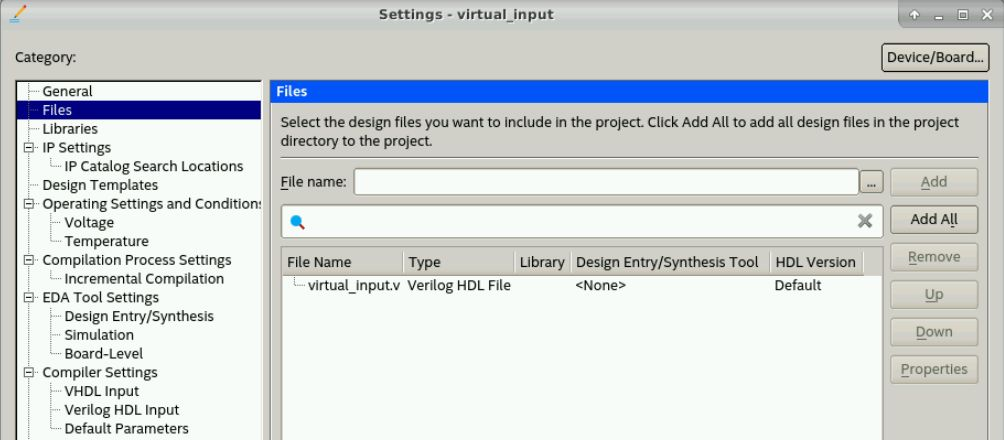
\includegraphics[width=0.8\textwidth]{img/files-quartus.jpg}
    \caption{\label{ref:files-quartus}Janela de inclusão de arquivos no projeto.}
    \end{figure}
    
    \item O componente do módulo \verb|virtual-input| pode ser incluído em um arquivo de diagrama de blocos clicando com o botão direito em um espaço vazio do esquemático e navegando para \textit{Insert}\verb|->|\textit{Symbol}, expandindo a biblioteca em \verb|/opt/[...]| e clicando duas vezes no item \verb|virtual_input|. Feito isso basta conectar o bloco com as entradas de seu projeto.
    
    \begin{figure}[H]
    \centering
    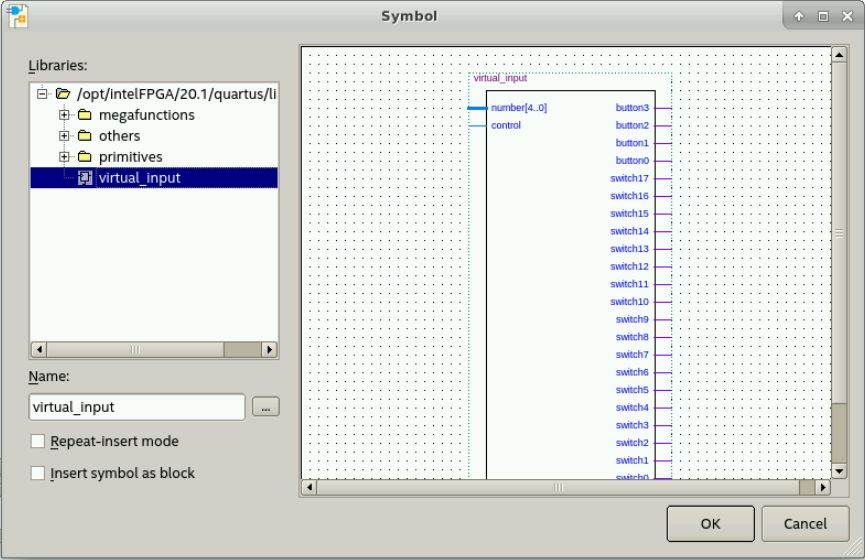
\includegraphics[width=0.8\textwidth]{img/block-quartus.jpg}
    \caption{\label{ref:block-quartus}Inclusão do dispositivo no arquivo de esquemático.}
    \end{figure}
    
    \item Para mapeamento dos pinos do módulos incluímos o arquivo \verb|virtual_input_pins.csv|, que pode ser importado para o projeto pelo menu \textit{Assignments}\verb|->|\textit{Import Assignments}. Na janela aberta basta selecionar o arquivo e clicar em \textit{OK}. Tentamos sempre manter o arquivo atualizado de acordo com a organização atual dos pinos, mas caso ocorram problemas com o mapeamento por favor contate o professor responsável.
    
    \begin{figure}[H]
    \centering
    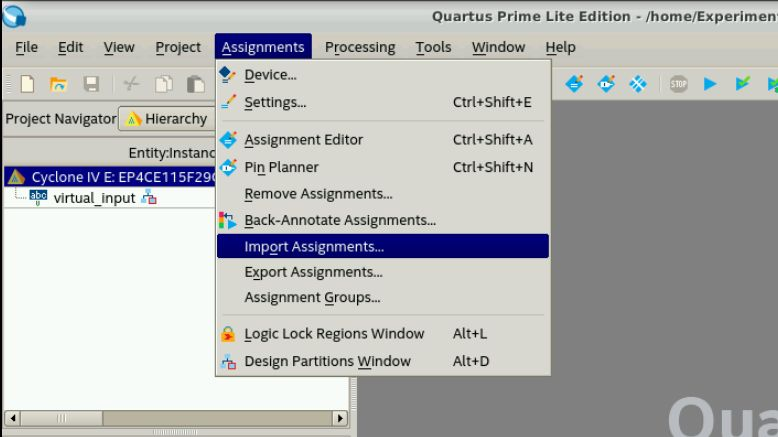
\includegraphics[width=0.8\textwidth]{img/pins-quartus.jpg}
    \caption{\label{ref:pins-quartus}Menu para importação de mapeamento.}
    \end{figure}
    
\end{enumerate}
Feito isso o projeto está pronto para ser compilado e operado virtualmente.

\section{Apresentação do Painel Virtual}
O programa ao iniciar apresenta os botões (no momento desativados) correspondentes aos recursos da placa, além de um display de mensagens e uma barra de menus.

\begin{figure}[H]
    \centering
    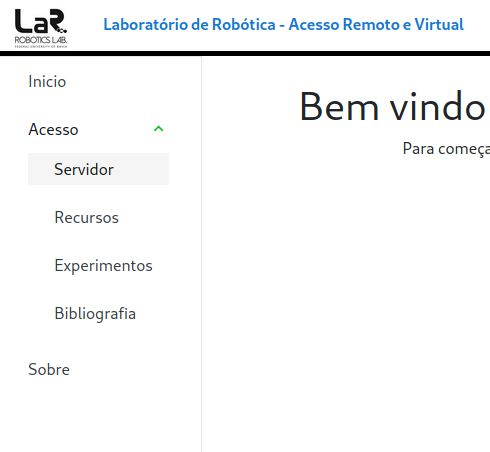
\includegraphics[width=0.6\textwidth]{img/site-lar.jpg}
    \caption{\label{ref:fig1}Tela inicial do programa.}
\end{figure}

No menu \textit{File} existem opções para iniciar o Quartus e o Cheese (aplicativo de câmera), para programação e visualização da placa, além de um botão para reiniciar o serviço JTAG (explicado mais adiante) e um para fechar o programa.

Enquanto não se conectar com um dispositivo serial, todos os botões continuarão desativados.
A conexão pode ser feita através do menu \textit{Devices}, que lista todos os dispositivos serial disponíveis no computador.
Ao clicar em um deles será iniciado processo de pareamento.
Para atualizar a lista basta clicar no botão \textit{Refresh}, caso ocorra alguma mudança nos dispositivos.

\section{Operação do Painel de Controle Virtual}
Antes de prosseguir com os passos abaixo certifique-se de que câmera e Quartus estejam iniciados, para a visualização e programação da placa, e que seu projeto no Quartus já foi preparado para operação remota conforme instruído na Seção 3 deste documento.

\begin{enumerate}[font=\bfseries]
    \item Através do menu \textit{Devices} conecte o Painel de Controle Virtual ao dispositivo Arduino presente. A conexão estará feita quando houver mensagem de confirmação positiva, e durará até ser fechada pelo usuário ou houver inatividade por mais de 10 minutos.

    \item Ligue a placa pelo botão POW agora disponível, e observe pela câmera.
    Os outros botões se tornarão disponíveis, mas não terão efeito enquanto a placa não for programada pelo Quartus.
    O botão POW tem um delay de aproximadamente 20 segundos entre ativações.

    \item Abra o \textit{Programmer} pelo menu \textit{Tools} do Quartus, selecione o USB Blaster na janela de dispositivos de transmissão* e inicie a programação da placa.
    
    \begin{figure}[H]
    \centering
    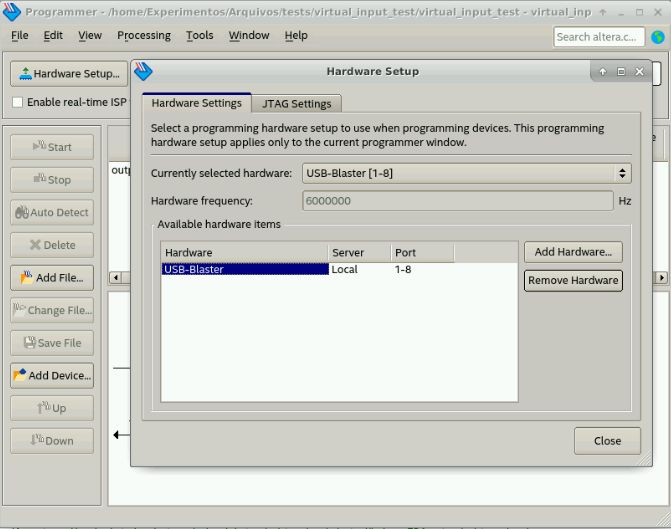
\includegraphics[width=0.8\textwidth]{img/usb-quartus.jpg}
    \caption{\label{ref:usb-quartus}Janela de seleção de dispositivos para programação.}
    \end{figure}

    \item Feita a programação basta clicar nos botões do Painel de Controle Virtual para enviá-los à placa, com visualização da operação pela câmera. Após 10 minutos de uso a DE2-115 desligará automaticamente para resfriamento.

    \item Terminados os testes, a placa pode ser desligada pelo botão POW e desconectada pelo menu \textit{Devices}, clicando na conexão atual. Feito isso, basta fechar o programa.
    
    \begin{figure}[H]
    \centering
    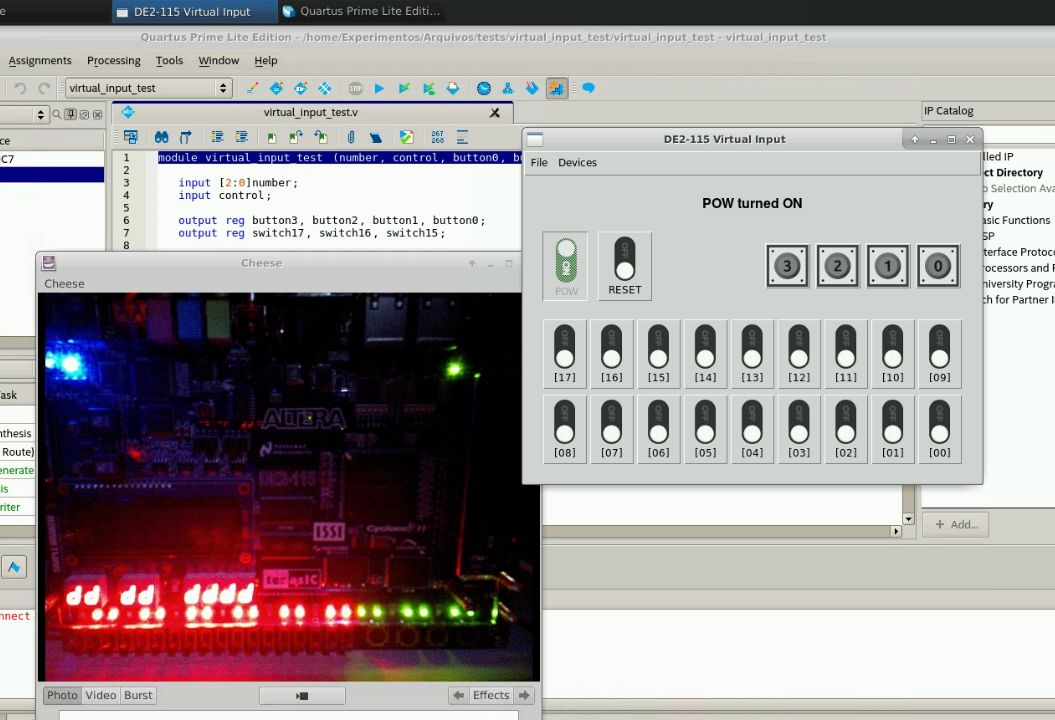
\includegraphics[width=0.9\textwidth]{img/operacao.jpg}
    \caption{\label{ref:operacao}Sessão virtual com Painel de Controle, Câmera e Quartus operando ao mesmo tempo.}
    \end{figure}
    
\end{enumerate}

\subparagraph{*OBS.} Caso o USB Blaster não conste na lista de dispositivos disponíveis para programação, feche a janela de dispositivos e abra novamente depois de alguns segundos, pois o botão POW reinicia o serviço de verificação de design JTAG e ele demora um pouco para abrir.
Caso mesmo depois de algumas tentativas o dispositivo ainda não apareça na lista ou a programação falhe, reinicie o JTAG pelo menu File.


\end{document}
